\section{結果と考察}

\subsection{評価方法}

風味を感じさせる四つの種類の中に香りが入っているゼリーを食べてもらい風味の感じ方を検
証する.システムにより一瞬でも風味を想起しか確認するために
4段階評価(1:全く感じない~4:すごく感じる)で変化の
度合いを調査する.さらに,自由記述でコメントを記入してもらうこととした.アンケートの回
答は風邪などひいておらず,嗅覚,味覚が正常な状態である6名の被験者を用意した.


\begin{figure}[b]
    \centering
    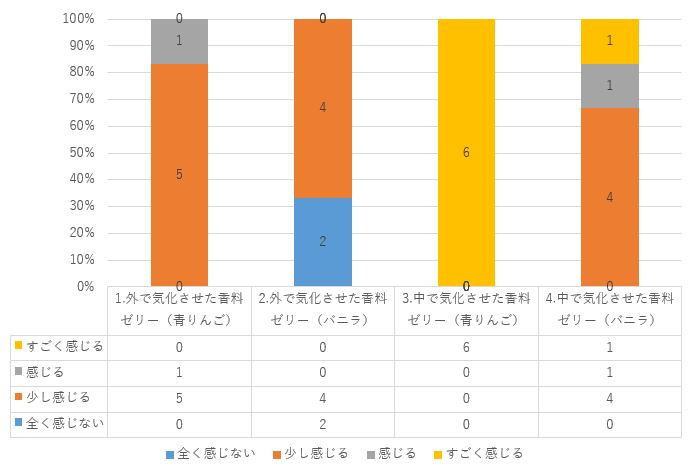
\includegraphics[width = 1.0\columnwidth]{gurafu1.JPG}
    \caption{風味の感じ方アンケート結果}
    \label{gurafu}
  \end{figure}


\subsection{実験結果と考察}

アンケート結果を図\ref{gurafu}に示した.
気化した香りを入れた場合の香りは,青りんごのVapeのリキッドとバニラエッセンス二つと
も少し感じたが多数であった.これは,気化した香りを入れた仕組みでは香りの量が少なく風味
を感じることが難しいという結果になった.


また,青りんごのVapeリキッドにおける評価は全員がすごく風味を感じたという結果であっ
た.バニラエッセンスは少し感じたという人が多数であった.これは香りが強いVapeのリキッ
ドは口内から鼻に抜ける風味を感じやすいと思われる.一方バニラエッセンスは香りが分かりに
くいため少し感じづらい結果になったと考える.これは,リキッドをゼリーの中で気化させる仕
組みが有効であったと言える.このことから,風味の感じ方に関しては気化した香りを入れるよりも,
ゼリーの中で気化させ香りを充満させる方が優位性が高いのではないかと考えられる.


自由記述では,「青りんごの香りが口の中から鼻に抜けるのを感じた」「味がないとおいしくは
ない」「ガムのような味」と言った様々な意見が得られた.


これらの結果から,レトロネーザルの嗅覚における影響に対しての仮説が生まれた.それは,
一つ目に青りんごのような風味を想像しやすい香りの方が風味を感じやすいのではないかという
考察が生まれた.バニラは普段口にする際,香りだけではなく甘い味がついていることがほとん
どのため香りだけで判断することが難しいと考えられる.


二つ目に,気化する量がカギになっているのではないかという仮説が生まれた.今回予備実験
で風味をあまり感じることが難しかったため,気化しやすく,香りが強いVapeのリキッドを使用
した.そのため,ゼリー内で気化した香りの量が増え,風味を感じやすくなったと考えられる.